% \section{Technologien}
% \label{sec:technologien}
%     Die bereits angesprochene Kommunikation und Vernetzung zwischen Geräten basiert im Allgemeinen auf 
%     diversen Protokollen. Um diese Datenbewegung und Kommunikation besser verstehen zu können, werden im 
%     Folgenden bekannte Protokolle erwähnt und aufgeführt und eines der meist verwendeten näher betrachtet. 
%     Um einen Vergleich herzustellen, wird ein vergleichbares Protokoll betrachtet. Diese werden dann zum 
%     Abschluss gegenübergestellt. 

%     \subsection{Übertragungsmethoden}
%     \label{subsec:netzwerkprotokolle}
%     Allgemein gibt es im Bereich des \acl{SH} mehrere Methoden und Möglichkeiten, die Objekte miteinander zu vernetzen. 
%     Unter dessen gehören Protokolle über Bluetooth, Ethernet, WLAN, Bussysteme, Funk und Stromleitung. 
%     Diese werden Abhängig von den Herstellern eingesetzt. Proprietäre Systeme funktionieren nur über eine 
%     Übertragungsmethode. So erzwingen die Hersteller die Nutzung einer Produktlinie, bzw. den Kauf einer 
%     einheitlichen Lösung. Geräte die die Möglichkeiten besitzen über mehrere Protokolle 
%     zu kommunizieren sind flexibler einsetzbar und mit mehreren Plattformen und Geräten kompatibel.
%     Grundlegend werden mit diesen Übertragungsmethoden Netzwerke erstellt, über das die Geräte in einem \acl{SH} kommunizieren können.
    % Die populärsten werden in folgender Tabelle aufgelistet\footnote{Auswahl von derzeit verwendeten Übertragungsmethoden. \url{https://de.wikipedia.org/wiki/Smart_Home\#Übertragungsmethoden} Abgerufen am 02.04.2022}: 
    \begin{table}[hbt!]
        \begin{center}
            \begin{tabular}{| p{3.25cm} | p{3.25cm} | p{3.25cm} | p{3.25cm} |}
                \hline
                    \textbf{Technologie} & \textbf{Übertragung} & \textbf{Frequenzbereich (Funk)} & \textbf{Proprietär} \\
                \hline
                    ZigBee & Funk & 2,4 GHz, 868 MHz & Nein \\ 
                \hline
                    Z-Wave & Funk & 868 MHz & Nein \\ 
                \hline
                    HomeMatic & Funk / Datenleitung & 868,3 MHz & Ja \\
                \hline
                    KNX & Funk / Strom- und Datenleitung & 868 MHz / - & Nein / Ja (Datenleitung als Gesamtsystem) \\
                \hline
                    Wi-Fi / WLAN & Funk & 2,4 - 5 GHz & Nein \\
                \hline 
                    Bluetooth & Funk & 2,4 GHz & Nein \\
                \hline
                    io-homecontrol & Funk & 868-870 MHz & Ja \\
                \hline
            \end{tabular}
        \end{center}
        \caption{Übertragungsmethoden des Smart Home}
        \label{tab:protocolsSH}
    \end{table}
    Die Auflistung der zum aktuellen Zeitpunkt am meist verwendeten Übertragungsmethoden dient 
    lediglich als Einblick, damit eine große Gesamtübersicht der Technologien und der Thematik \acl{SH} entsteht. 
    Demnach wird im Rahmen dieser Arbeit das Thema oberflächlich erläutert und nicht ausführlich vertieft.
    %ZigBee? Erläuterung etwas detaillierter?

    % https://www.bigdata-insider.de/so-laeuft-der-datenaustausch-zwischen-edge-und-cloud-a-1097887/ 

    \subsection{MQTT}
    \label{subsec:mqtt}
        Das \ac{MQTT}-Protokoll ist eines der ältesten offenen Netzwerk- und Nachrichtenprotokolle der 
        \ac{MtoM}-Kommunikation. 
        Dies wurde 1999 von IBM Mitarbeiter Andy Stanford-Clark\footnote{Informationen zu Herrn Stanford-Clark \url{https://stanford-clark.com} Abgerufen am 12.04.2022} 
        und von Cirrus Link Solutions Mitarbeiter Arlen Nipper\footnote{Informationen zu Herrn Nipper \url{https://www.inductiveautomation.com/resources/podcast/the-coinventor-of-mqtt-arlen-nipper-from-cirrus-link-solutions} Abgerufen am 12.04.2022} 
        entwickelt. Die Technologie ermöglicht die Übertragung von Messdaten, sogenannten Telemetriedaten, in Form von 
        Nachrichten zwischen Maschinen und Geräten. Die erzeugten Messdaten durch beispielsweise Sensoren und Aktoren 
        können durch ihre minimale Größe und die kompakte Form des Protokolls in einem kleinen Datenpaket auch bei 
        hoher Verzögerung oder bei beschränktem Netzwerk übertragen werden \cite{Naik2017}. \acs{MQTT} ist ein 
        klassisches Client-Sever-Protokoll, welches nach dem \textit{Publish/Subscribe} Kommunikationsmodell 
        entwickelt wurde. Ein \acs{MQTT}-Client veröffentlicht Nachrichten an einen \acs{MQTT}-Server, den sogenannten 
        \acs{MQTT}-Broker. Diese können von anderen Clients abonniert oder auf dem Broker für zukünftige Abonnements 
        aufbewahrt werden. Jede erzeugte Nachricht wird an eine Adresse veröffentlicht, die als Thema, im Englischen \textit{Topic}, 
        bezeichnet wird \cite{Naik2017}. \acs{MQTT}-Clients können mehrere Topics abonnieren und erhalten jede Nachricht, die an das jeweilig abonnierte Topic gesendet wird. 
        \\
        Die Leichtgewichtigkeit des Protokolls ermöglicht es, die Nachrichten bei eingeschränkter Netzwerkverfügbarkeit zu 
        übermitteln. Ausschlaggebend dafür ist das binär-basierte Protokoll, welches normalerweise einen festen Header von 
        zwei Bytes mit kleinen Nachrichtennutzlasten von maximal bis zu einer Grüße von 256 MB \cite{Naik2017} enthält. Grundlegend 
        ist \acs{MQTT} auf der Basis des Transportprotokoll \ac{TCP} aufgebaut und nutzt zur Verstärkung der Sicherheit die 
        \ac{TLS}/\ac{SSL}-Verschlüsselung. Dadurch sind Client und Broker mit ihrer Kommunikation verbindungsorientiert.  
        Die Anwendung von \acs{MQTT} im Bereich des \acl{SH} zeichnet sich durch die Möglichkeit aus, große Netzwerke mit 
        vielen kleineren Geräten, die von einem Backend-Server, bzw. dem Backend-System überwacht und gesteuert werden müssen, zu 
        betreiben. Dennoch ist es nicht für Multicast-Daten oder Übertragungen von Gerät zu Gerät ausgelegt. Die Nutzbarkeit 
        von \acs{MQTT} ist aufgrund der wenigen Steueroptionen und der Einfachheit des Messaging-Protokolls sehr simplen und 
        leichtgewichtig \cite{Naik2017}. 
        \\
        \linebreak
        Ein interessanter Aspekt des \acs{MQTT}-Brokers ist, dass er die gesamte Datenlage seiner Kommunikationspartner aufbewahrt und 
        so die Option bietet, zusätzlich als Zustand-Datenbank betrieben werden kann. Dadurch können weniger leistungsfähige Geräte 
        mit einem \acs{MQTT}-Broker verbunden werden, bei denen die Geräte Befehle und Daten entgegennehmen können, zugleich aber ein 
        komplexeres Lagebild auf dem Broker entsteht. So können Daten an einen leistungsfähigeren Kommunikationspartner 
        weitergeleitet und dort ausgewertet werden.\footnote{\url{https://mqtt.org} Abgerufen am 13.04.2022}
        \\
        Mit diesem Aspekt können durch das \acl{MQTT} Protokoll Automatisierungslösungen geschaffen werden und findet dadurch im 
        Segment \acs{IoT} und \acl{SH} einfache Verwendung und dementsprechend eine große und schnelle Verbreitung. 
        \\
        \linebreak
        Zusammengefasst ist der \acs{MQTT}-Broker die Kommunikationsschnittstelle der \acl{SH}-Geräte und der \acl{SH}-Plattform. 
        Alle Kommunikationspartner können so Informationen (Nachrichten / Messages) auf bestimmte Topics (Endpunkten) senden und 
        diese abonnieren (publish / subscribe). 

        \subsubsection*{Publish/Subscribe Kommunikationmodell}
        \label{subsubsec:pubsub}
            Das Prinzip des Publish/Subscribe Kommunikationsmodells besteht darin, dass Komponenten, die daran 
            interessiert sind, bestimmte Informationen zu konsumieren, ihr Interesse anmelden \cite{Hunkeler2008}. Dieser Vorgang wird als 
            Abonnement (subscription) bezeichnet. Geräte, die an dem Vorgang oder an bestimmten Informationen interessiert sind, 
            werden als Abonnenten (subscriber) definiert. Im Gegenzug können Geräte und Komponenten bestimmte Informationen produzieren und 
            diese veröffentlichen (publish) und an bestimmte Abonnenten weitergeben. Diese Vermittlung der Informationen zwischen 
            Herausgeber (publisher) und Abonnent (subscriber) erfolgt über den Markler (broker), dieser koordiniert sämtlichen Abonnements. 
            Alle Abonnent müssen sich explicit bei dem Broker anmelden, um die Informationen zu erhalten \cite{Hunkeler2008}. 
            \begin{figure}[hbt!]
                \centering
                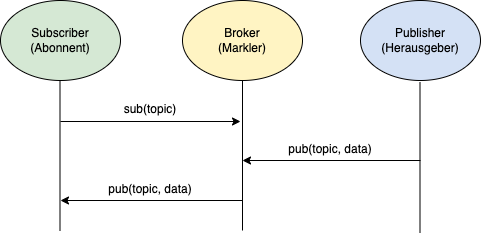
\includegraphics[width=12cm,height=12cm,keepaspectratio]{images/sub-model.drawio.png}
                \caption{Themenbasiertes Pub/Sub Kommunikationsmodell \cite{Hunkeler2008}}
                \label{pic:pub-sub-model}
            \end{figure}
            \\
            Dieses Prinzip ist ein essentieller Bestandteil des \acs{MQTT}-Protokolls. Im Folgenden wird ein Beispiel aufgezeigt, welches 
            die Kommunikation über das Publish/Subscribe Modell darstellt.
            
            \subsubsection*{Beispiel}
            \label{subsubsec:pubsub-example}
            Damit am Beispiel der Steuerzentrale, die im Rahmen dieser Arbeit konzipiert und prototypisch implementiert wird, 
            ein Prozess gestartet werden kann, müssen bestimmte Ereignisse durch \acs{MQTT} Nachrichten eintreten. Das hier 
            verwendete Beispiel ist das Öffnen einer Büroeingangstür. Hierbei wird von einem Relais an der Tür, welches das Türschloss steuert, eine Nachricht and den \textit{Broker} herausgegeben:
            \\
            \begin{lstlisting}[language=Java, frame=lines, xleftmargin=\parindent, style=algoBericht, label={code:entity}, captionpos=b, caption={Erzeugung und Veröffentlichung einer Nachricht}]
                publish -topic: Buero/Tuer/Zustand -message: "offen"
            \end{lstlisting}
            Diese Nachricht wird von der Steuerzentrale konsumiert und weiterverarbeitet. Damit der Informationskanal (topic) 
            über die Steuerzentrale verfügbar ist, muss dieser Kanal konsumiert werden: 
            \\
            \begin{lstlisting}[language=Java, frame=lines, xleftmargin=\parindent, style=algoBericht, label={code:entity}, captionpos=b, caption={Empfang und Konsum einer Nachricht}]
                subscribe -topic: Buero/Tuer/Zustand
            \end{lstlisting}
            Mit der empfangenen Nachricht kann dann über die Steuerzentrale ein Prozess, welcher vorab als Regel implementiert wurde, ausgelöst werden. Beispielsweise eine Durchsage im Büro, dass die Tür offen steht, bzw. eine Person eintritt.
    \pagebreak
    \subsection{AMQP}
    \label{subsec:amqp}
        Das \ac{AMQP}-Protokoll ist ebenso ein leichtgewichtiges \acs{MtoM}-Protokoll, welches im Jahre 2003 von John O\'Hara JPMorgan Chase 
        in London, Großbritannien, entwickelt wurde \cite{Naik2017}. Der Fokus diesen Protokolls liegt auf der Unternehmens-Messaging Ebene 
        und legt hohen Wert auf die Zuverlässigkeit, Sicherheit, Bereitstellung und Interoperabilität der Kommunikation. \acs{AMQP} 
        unterstützt neben der Publish/Subscribe- auch die Request/Response Architektur. Es bietet eine breite Palette von 
        Funktionen im Zusammenhang mit Messaging, wie z. B. zuverlässiges Queuing, themenbasiertes Publish-and-Subscribe-Messaging, 
        flexibles Routing und Transaktionen \cite{Naik2017}. Das Kommunikationsmodell nach dem \acs{AMQP} Standard erfordert, dass der 
        Herausgeber (publisher) oder der Empfänger (subscriber) einen \textit{Austausch (exchange)} mit einem bestimmten Namen generiert 
        und diesen dann sendet \cite{Naik2017}. Die beiden Komponenten, Empfänger und Herausgeber, nutzen den Namen des Austausch, um eine 
        Verbindung aufzubauen. Der Empfänger erstellt darauf eine Warteschlange (queue) und hängt diese an den Austausch an. Nachrichten, die 
        über diese Verbindung ausgetauscht werden, müssen über einen gesonderten Prozess (binding) mit der Warteschlange abgeglichen werden 
        \cite{Naik2017}.
        \\ 
        Das binäre Protokoll \acs{AMQP} erfordert einen Header von acht Byte mit Nachrichtennutzlasten, die die Größe der Nachricht ist abhängig 
        von dem Broker, bzw. dem Server. Die verbindungsorientierte Kommunikation von \acs{AMQP} basiert auf dem Standard-Transportprotokoll 
        \acs{TCP} und zur Sicherheit auf dem \acs{TLS}/\acs{SSL}-Protokoll. Ein Kernmerkmal des \acs{AMQP} Kommunikationsmodells ist die 
        Zuverlässigkeit \cite{Naik2017}. 
        \\
        \linebreak
        Neben den beiden aufgeführten Kommunikationsmodellen gibt es noch weitere, darunter das klassische \ac{HTTP} und das \ac{COAP}, die allerdings im Rahmen dieser Arbeit nicht weiter ausgeführt werden. 
        %Der Fokus in dieser Arbeit liegt auf dem \acs{MQTT}-Protokoll. 
        
        %Vergleich in den Anhang packen??
        %\subsubsection*{Vergleich von MQTT und AMQP}
        %\label{subsubsec:mqtt-vs-amqp}
        %\begin{table}[hbt!]
        %    \begin{center}
        %        \begin{tabular}{| p{3.25cm} | p{6cm} | p{6cm} | }
        %            \hline
        %                \textbf{Kriterium} & \textbf{MQTT} & \textbf{AMWP}\\
        %            \hline
        %                Jahr & 1999 & 2003 \\ 
        %            \hline
        %                Architektur & Client/Broker, & Client/Broker Client/Server \\ 
        %            \hline
        %                Abstraktion & Publish/Subscribe & Publish/Subscribe Request/response \\ 
        %            \hline
        %                Header Größe & 2 Byte,  & 8 Byte \\ 
        %            \hline
        %                Nachrichtengröße & max. 265 MB & Abhängig von Broker/Server \\ 
        %            \hline 
        %                Semantik / Methoden & Connect, Disconnect, Publish, Subscribne, Unsubscribe, Close & Consume, Deliver, Publish, Get, Select, Ack, Delete, Nack, Recover, Reject, Open, Close \\
        %            \hline
        %                Zwischenspeicher (Cache) und Proxy & Teilweise & Ja \\
        %            \hline
        %                Standards & OASIS, Eclipse Foundation  & OASIS, ISO/IEC \\ 
        %            \hline
        %                Transport-Protokoll & TCP, & TCP, SCTP \\
        %            \hline
        %                Sicherheit & TLS/SSL & TLS/SSL \\ 
        %            \hline
        %                Standard-Port & 1883/8883 (TLS/SSL) & 5671 (TLS/SSL), 5672 \\
        %            \hline
        %                Format & binär  & Binär \\ 
        %            \hline
        %                Lizenzmodell & Open Source & Open Source \\
        %            \hline
        %                Support & IBM, Facebook, Eurotech, Cisco, Red Hat Amazon (AWS) etc. & Microsoft, JP Morgan, Bank of America, Barclays, Goldman Sachs Credit Suisse \\ 
        %            \hline
        %        \end{tabular}
        %    \end{center}
        %    \caption{Vergleich von MQTT und AMQP \cite{Naik2017}}
        %    \label{tab:mqtt-vs-amqp}
        %\end{table}
        
        
        %Dadurch wird die Konfiguration und Einsetzbarkeit der Technologie komplexer im Gegenzug zu MQTT


        % Vergleich zu MQTT

    
    % Überlegen, bzw. abwarten, ob das benötigt wird.... 
    %\subsection{Raspberry Pi}
    %\label{subsec:raspberrypi} 
